\documentclass[11pt]{article}
\makeatletter\if@twocolumn\PassOptionsToPackage{switch}{lineno}\else\fi\makeatother

      \makeatletter
\usepackage{wrapfig}
\newcounter{aubio}

\long\def\bioItem{%
\@ifnextchar[{\@bioItem}{\@@bioItem}}

\long\def\@bioItem[#1]#2#3{
 \stepcounter{aubio}
 \expandafter\gdef\csname authorImage\theaubio\endcsname{#1}
 \expandafter\gdef\csname authorName\theaubio\endcsname{#2}
 \expandafter\gdef\csname authorDetails\theaubio\endcsname{#3}
}

\long\def\@@bioItem#1#2{
 \stepcounter{aubio}
 \expandafter\gdef\csname authorName\theaubio\endcsname{#1}
 \expandafter\gdef\csname authorDetails\theaubio\endcsname{#2}
}

\newcommand{\checkheight}[1]{%
  \par \penalty-100\begingroup%
  \setbox8=\hbox{#1}%
  \setlength{\dimen@}{\ht8}%
  \dimen@ii\pagegoal \advance\dimen@ii-\pagetotal
  \ifdim \dimen@>\dimen@ii
    \break
  \fi\endgroup}

\def\printBio{%
  \@tempcnta=0
   \loop
     \advance \@tempcnta by 1
     \def\aubioCnt{\the\@tempcnta}
     \setlength{\intextsep}{0pt}%
     \setlength{\columnsep}{10pt}%
     \newbox\boxa%
     \setbox\boxa\vbox{\csname authorDetails\aubioCnt\endcsname}
     \expandafter\ifx\csname authorImage\aubioCnt\endcsname\relax%
      \else%
       \checkheight{\includegraphics[height=1.25in,width=1in,keepaspectratio]{\csname authorImage\aubioCnt\endcsname}}
        \begin{wrapfigure}{l}{25mm}
         \includegraphics[height=1.25in,width=1in,keepaspectratio]{\csname authorImage\aubioCnt\endcsname}%height=145pt
        \end{wrapfigure}\par
      \fi
     {\parindent0pt\textbf{\csname authorName\aubioCnt\endcsname}\csname authorDetails\aubioCnt\endcsname \par\bigskip%
     \expandafter\ifx\csname authorImage\aubioCnt\endcsname\relax\else%
      \ifdim\the\ht\boxa < 90pt\vskip\dimexpr(90pt -\the\ht\boxa-1pc)\fi%
     \fi}%for adding additional vskip for avoiding image overlap.
      \ifnum\@tempcnta < \theaubio
   \repeat
   }

\makeatother

      



\usepackage{amsfonts,amssymb,amsbsy,latexsym,amsmath,tabulary,graphicx,times,xcolor}
\usepackage[utf8x]{inputenc}
\usepackage{fancyhdr}
\def\NormalBaseline{\def\baselinestretch{1.1}}
\makeatletter
\def\hlinewd#1{%
  \noalign{\ifnum0=`}\fi\hrule \@height #1%
  \futurelet\reserved@a\@xhline}
\def\tbltoprule{\hlinewd{.8pt}}%\\[-10pt]}
\def\tblbottomrule{\hlinewd{.8pt}}
\def\tblmidrule{\hline\noalign{\vspace*{2pt}}}

\def\@shorttitle{\@empty}
\def\shorttitle#1{\gdef\@shorttitle{#1}}

\fancypagestyle{custom}{
\fancyhf{}
\fancyhead[C]{\@shorttitle}
\fancyhead[R]{\thepage}
\fancyfoot[C]{}
\renewcommand\headrulewidth{0.4pt}
\renewcommand\footrulewidth{0pt}
}
\fancypagestyle{plain}{
\fancyhf{}
\renewcommand\headrulewidth{0.4pt}
}


\makeatother

\usepackage{times}

\usepackage[a4paper,margin=2.5cm,headsep=.7cm,headheight=18pt,top=3cm,footnotesep=1.5\baselineskip]{geometry}
\usepackage{caption}
\captionsetup[figure]{labelfont=bf,labelsep=newline,justification=centerlast,labelfont={small,sc,bf},font=small,aboveskip=.3\baselineskip}

\captionsetup[table]{labelfont=bf,labelsep=newline,justification=centerlast,labelfont={small,sc,bf},font=small,aboveskip=.3\baselineskip}
\linespread{1.5}

\setcounter{totalnumber}{4}
\def\topfraction{0.9}
\def\bottomfraction{0.4}
\def\floatpagefraction{0.8}
\def\textfraction{0.1}
\widowpenalty 10000
\clubpenalty 10000
\makeatletter
\setlength\intextsep   {1.5\baselineskip \@plus 2\p@ \@minus 2\p@}
\makeatother

  
%%%%%%%%%%%%%%%%%%%%%%%%%%%%%%%%%%%%%%%%%%%%%%%%%%%%%%%%%%%%%%%%%%%%%%%%%%
% Following additional macros are required to function some 
% functions which are not available in the class used.
%%%%%%%%%%%%%%%%%%%%%%%%%%%%%%%%%%%%%%%%%%%%%%%%%%%%%%%%%%%%%%%%%%%%%%%%%%
\usepackage{url,multirow,morefloats,floatflt,cancel,tfrupee}
\makeatletter


\AtBeginDocument{\@ifpackageloaded{textcomp}{}{\usepackage{textcomp}}}
\makeatother
\usepackage{colortbl}
\usepackage{xcolor}
\usepackage{pifont}
\usepackage[nointegrals]{wasysym}
\urlstyle{rm}
\makeatletter

%%%For Table column width calculation.
\def\mcWidth#1{\csname TY@F#1\endcsname+\tabcolsep}

%%Hacking center and right align for table
\def\cAlignHack{\rightskip\@flushglue\leftskip\@flushglue\parindent\z@\parfillskip\z@skip}
\def\rAlignHack{\rightskip\z@skip\leftskip\@flushglue \parindent\z@\parfillskip\z@skip}

%Etal definition in references
\@ifundefined{etal}{\def\etal{\textit{et~al}}}{}


%\if@twocolumn\usepackage{dblfloatfix}\fi
\usepackage{ifxetex}
\ifxetex\else\if@twocolumn\@ifpackageloaded{stfloats}{}{\usepackage{dblfloatfix}}\fi\fi

\AtBeginDocument{
\expandafter\ifx\csname eqalign\endcsname\relax
\def\eqalign#1{\null\vcenter{\def\\{\cr}\openup\jot\m@th
  \ialign{\strut$\displaystyle{##}$\hfil&$\displaystyle{{}##}$\hfil
      \crcr#1\crcr}}\,}
\fi
}

%For fixing hardfail when unicode letters appear inside table with endfloat
\AtBeginDocument{%
  \@ifpackageloaded{endfloat}%
   {\renewcommand\efloat@iwrite[1]{\immediate\expandafter\protected@write\csname efloat@post#1\endcsname{}}}{\newif\ifefloat@tables}%
}%

\def\BreakURLText#1{\@tfor\brk@tempa:=#1\do{\brk@tempa\hskip0pt}}
\let\lt=<
\let\gt=>
\def\processVert{\ifmmode|\else\textbar\fi}
\let\processvert\processVert

\@ifundefined{subparagraph}{
\def\subparagraph{\@startsection{paragraph}{5}{2\parindent}{0ex plus 0.1ex minus 0.1ex}%
{0ex}{\normalfont\small\itshape}}%
}{}

% These are now gobbled, so won't appear in the PDF.
\newcommand\role[1]{\unskip}
\newcommand\aucollab[1]{\unskip}
  
\@ifundefined{tsGraphicsScaleX}{\gdef\tsGraphicsScaleX{1}}{}
\@ifundefined{tsGraphicsScaleY}{\gdef\tsGraphicsScaleY{.9}}{}
% To automatically resize figures to fit inside the text area
\def\checkGraphicsWidth{\ifdim\Gin@nat@width>\linewidth
	\tsGraphicsScaleX\linewidth\else\Gin@nat@width\fi}

\def\checkGraphicsHeight{\ifdim\Gin@nat@height>.9\textheight
	\tsGraphicsScaleY\textheight\else\Gin@nat@height\fi}

\def\fixFloatSize#1{}%\@ifundefined{processdelayedfloats}{\setbox0=\hbox{\includegraphics{#1}}\ifnum\wd0<\columnwidth\relax\renewenvironment{figure*}{\begin{figure}}{\end{figure}}\fi}{}}
\let\ts@includegraphics\includegraphics

\def\inlinegraphic[#1]#2{{\edef\@tempa{#1}\edef\baseline@shift{\ifx\@tempa\@empty0\else#1\fi}\edef\tempZ{\the\numexpr(\numexpr(\baseline@shift*\f@size/100))}\protect\raisebox{\tempZ pt}{\ts@includegraphics{#2}}}}

%\renewcommand{\includegraphics}[1]{\ts@includegraphics[width=\checkGraphicsWidth]{#1}}
\AtBeginDocument{\def\includegraphics{\@ifnextchar[{\ts@includegraphics}{\ts@includegraphics[width=\checkGraphicsWidth,height=\checkGraphicsHeight,keepaspectratio]}}}

\DeclareMathAlphabet{\mathpzc}{OT1}{pzc}{m}{it}

\def\URL#1#2{\@ifundefined{href}{#2}{\href{#1}{#2}}}

%%For url break
\def\UrlOrds{\do\*\do\-\do\~\do\'\do\"\do\-}%
\g@addto@macro{\UrlBreaks}{\UrlOrds}



\edef\fntEncoding{\f@encoding}
\def\EUoneEnc{EU1}
\makeatother
\def\floatpagefraction{0.8} 
\def\dblfloatpagefraction{0.8}
\def\style#1#2{#2}
\def\xxxguillemotleft{\fontencoding{T1}\selectfont\guillemotleft}
\def\xxxguillemotright{\fontencoding{T1}\selectfont\guillemotright}

\newif\ifmultipleabstract\multipleabstractfalse%
\newenvironment{typesetAbstractGroup}{}{}%

%%%%%%%%%%%%%%%%%%%%%%%%%%%%%%%%%%%%%%%%%%%%%%%%%%%%%%%%%%%%%%%%%%%%%%%%%%

\usepackage{natbib}




\usepackage{titlesec}
\usepackage[T1]{fontenc}
\setcounter{secnumdepth}{5}
 
\titleformat{\section}[hang]{\NormalBaseline\filright\large\bfseries}
{\large\thesection}
{10pt}
{}
[]
\titleformat{\subsection}[hang]{\NormalBaseline\filright\bfseries}
{\thesubsection}
{10pt}
{}
[]
\titleformat{\subsubsection}[hang]{\NormalBaseline\filright\bfseries\itshape}
{\upshape\thesubsubsection}
{10pt}
{}
[]
\titleformat{\paragraph}[runin]{\NormalBaseline\filright\bfseries}
{\theparagraph}
{10pt}
{}
[]
\titleformat{\subparagraph}[runin]{\NormalBaseline\filright\bfseries\itshape}
{\thesubparagraph}
{10pt}
{}
[]

\titlespacing{\section}{0pt}{1.5\baselineskip}{.2\baselineskip}  
\titlespacing{\subsection}{0pt}{1.5\baselineskip}{.2\baselineskip}  
\titlespacing{\subsubsection}{0pt}{1.5\baselineskip}{.2\baselineskip}  
\titlespacing{\paragraph}{0pt}{.5\baselineskip}{10pt}  
\titlespacing{\subparagraph}{0pt}{.5\baselineskip}{10pt}  
  

  




\usepackage{float}

\begin{document}



\renewcommand*\rmdefault{bch}\normalfont\upshape

\shorttitle{Class Assignment}

\date{}  

  
\title{\NormalBaseline\raggedright\bfseries Infrared Spectroscopy {\textemdash} Paper Review}
  \let\origthanks\thanks
\renewcommand\thanks[1]{\begingroup\let\rlap\relax\origthanks{#1}\endgroup}
\author{\hskip2pc\parbox{.95\textwidth}{\bfseries\large Antonio Osamu Katagiri Tanaka\textsuperscript{1}\thanks{E-mail: A01212611@itesm.mx}
      \\[3pt] 
    % Address
    \normalfont\itshape\NormalBaseline \textsuperscript{\upshape 1} 
    ITESM\unskip, \normalfont\itshape\NormalBaseline Av. Eugenio Garza Sada 2501 Sur\unskip, N.L.\unskip, Monterrey\unskip, Mexico}}
    
    
\maketitle 
\pagestyle{custom}

    
\section{Paper Review: Reflectance FT-IR spectroscopy as a viable option for textile fiber identification\unskip~\protect\cite{693772:16533873}}
Fourier Transform Infrared Spectroscopy (FTIR) plays an important role in the identification of textile fibers, due to the forensics and cultural heritage applications. Often samples are unique and/or highly valuable, therefore either extremely small samples or non-destructive characterization techniques are to be implemented during the analysis process. On the other hand, modern regenerated and synthetic fibers are very similar in morphology and are unable to be reliably characterized with microscopic visualization methods\unskip~\cite{693772:16533873}.

Attenuated Total Reflectance FTIR (ATR-FTIR) is the most popular characterization technique in the analyzes of textile fibers. However, ATR-FTIR requires the application of significant pressure to the textile sample which may damage the unique/valuable sample. Reflectance FTIR (r-FTIR) allows the analyzes of small parts of larger objects without sample removal or manipulation. Nevertheless, r-FTIR only works for flat surfaces\unskip~\cite{693772:16533873}.



\subsection{Chemicals and reagents}For the analysis, Peets et al. worked with 61 single-component textile fibers from 16 different types were used: wool, silk, cotton, linen, jute, sisal, viscose, acetate, lyocell, fiberglass, polyester, polyamide, polyacrylic, elastane, polyethylene and polypropylene. Textile samples were obtained from different companies from Estonia, fabric stores, and private collections\unskip~\cite{693772:16533873}.



\subsection{Instrumentation \& Method}For r-FTIR, samples were placed on a gold plate, which was also used as back- ground. ForATR-FTIR, the ATR objective was a conical germanium crystal with 60{\textendash}75\% sample pressure strength. To evaluate both techniques, the authors compare the r-FTIR spectra against the ATR-FTIR spectra for the same materials\unskip~\cite{693772:16533873}.



\subsection{Results}The r-FTIR vs. ATR-FTIR spectrum comparison revealed general similarity with small variations. In most cases, the absorbance bands in r-FTIR are wider, with wave numbers shifted to higher values and intensity peaks vary from the ATR-FTIR equivalents.  Peets et al.'s general conclusion states that the performance of r-FTIR is comparable to ATR-FTIR\unskip~\cite{693772:16533873}.

More specifically, r-FTIR works better than ATR-FTIR in the identification of polyamide-based fibers, but it's less successful in differentiating cellulose-based fibers. The authors presented a side-by-side r-FTIR vs. ATR-FTIR spectra comparison of the most common textile fibers, as shown in Figure~\ref{f-cbfac61d0782}. The figure implies that:


  
  \begin{enumerate}
  \item \relax r-FTIR spectra seem to contain more absorbance maxima compared to the ATR-FTIR technique. In particular in the region of $3000-4000 cm^{-1} $ the bands are wider and more intensive.
  \item \relax r-FTIR shits the bands toward higher wave numbers, compared to ATR-FTIR.
  \item \relax The characteristic $C-O $ stretching band of viscose (and cotton) near $1022 cm^{-1} $is easily identified in the ATR spectra, which has merged into a wide absorbance range in the r-FTIR spectra.
  \item \relax r-FTIR is discovered to better classify polyamide-based fibers (silk, wool, and synthetic polyamide) than ATR-FTIR\unskip~\cite{693772:16533873}.
  \end{enumerate}
  
\bgroup
\fixFloatSize{images/1e7c6525-a9ac-4ff7-a4ff-b7128f317966-ufig1_comparison.png}
\begin{figure*}[!htbp]
\centering \makeatletter\IfFileExists{images/1e7c6525-a9ac-4ff7-a4ff-b7128f317966-ufig1_comparison.png}{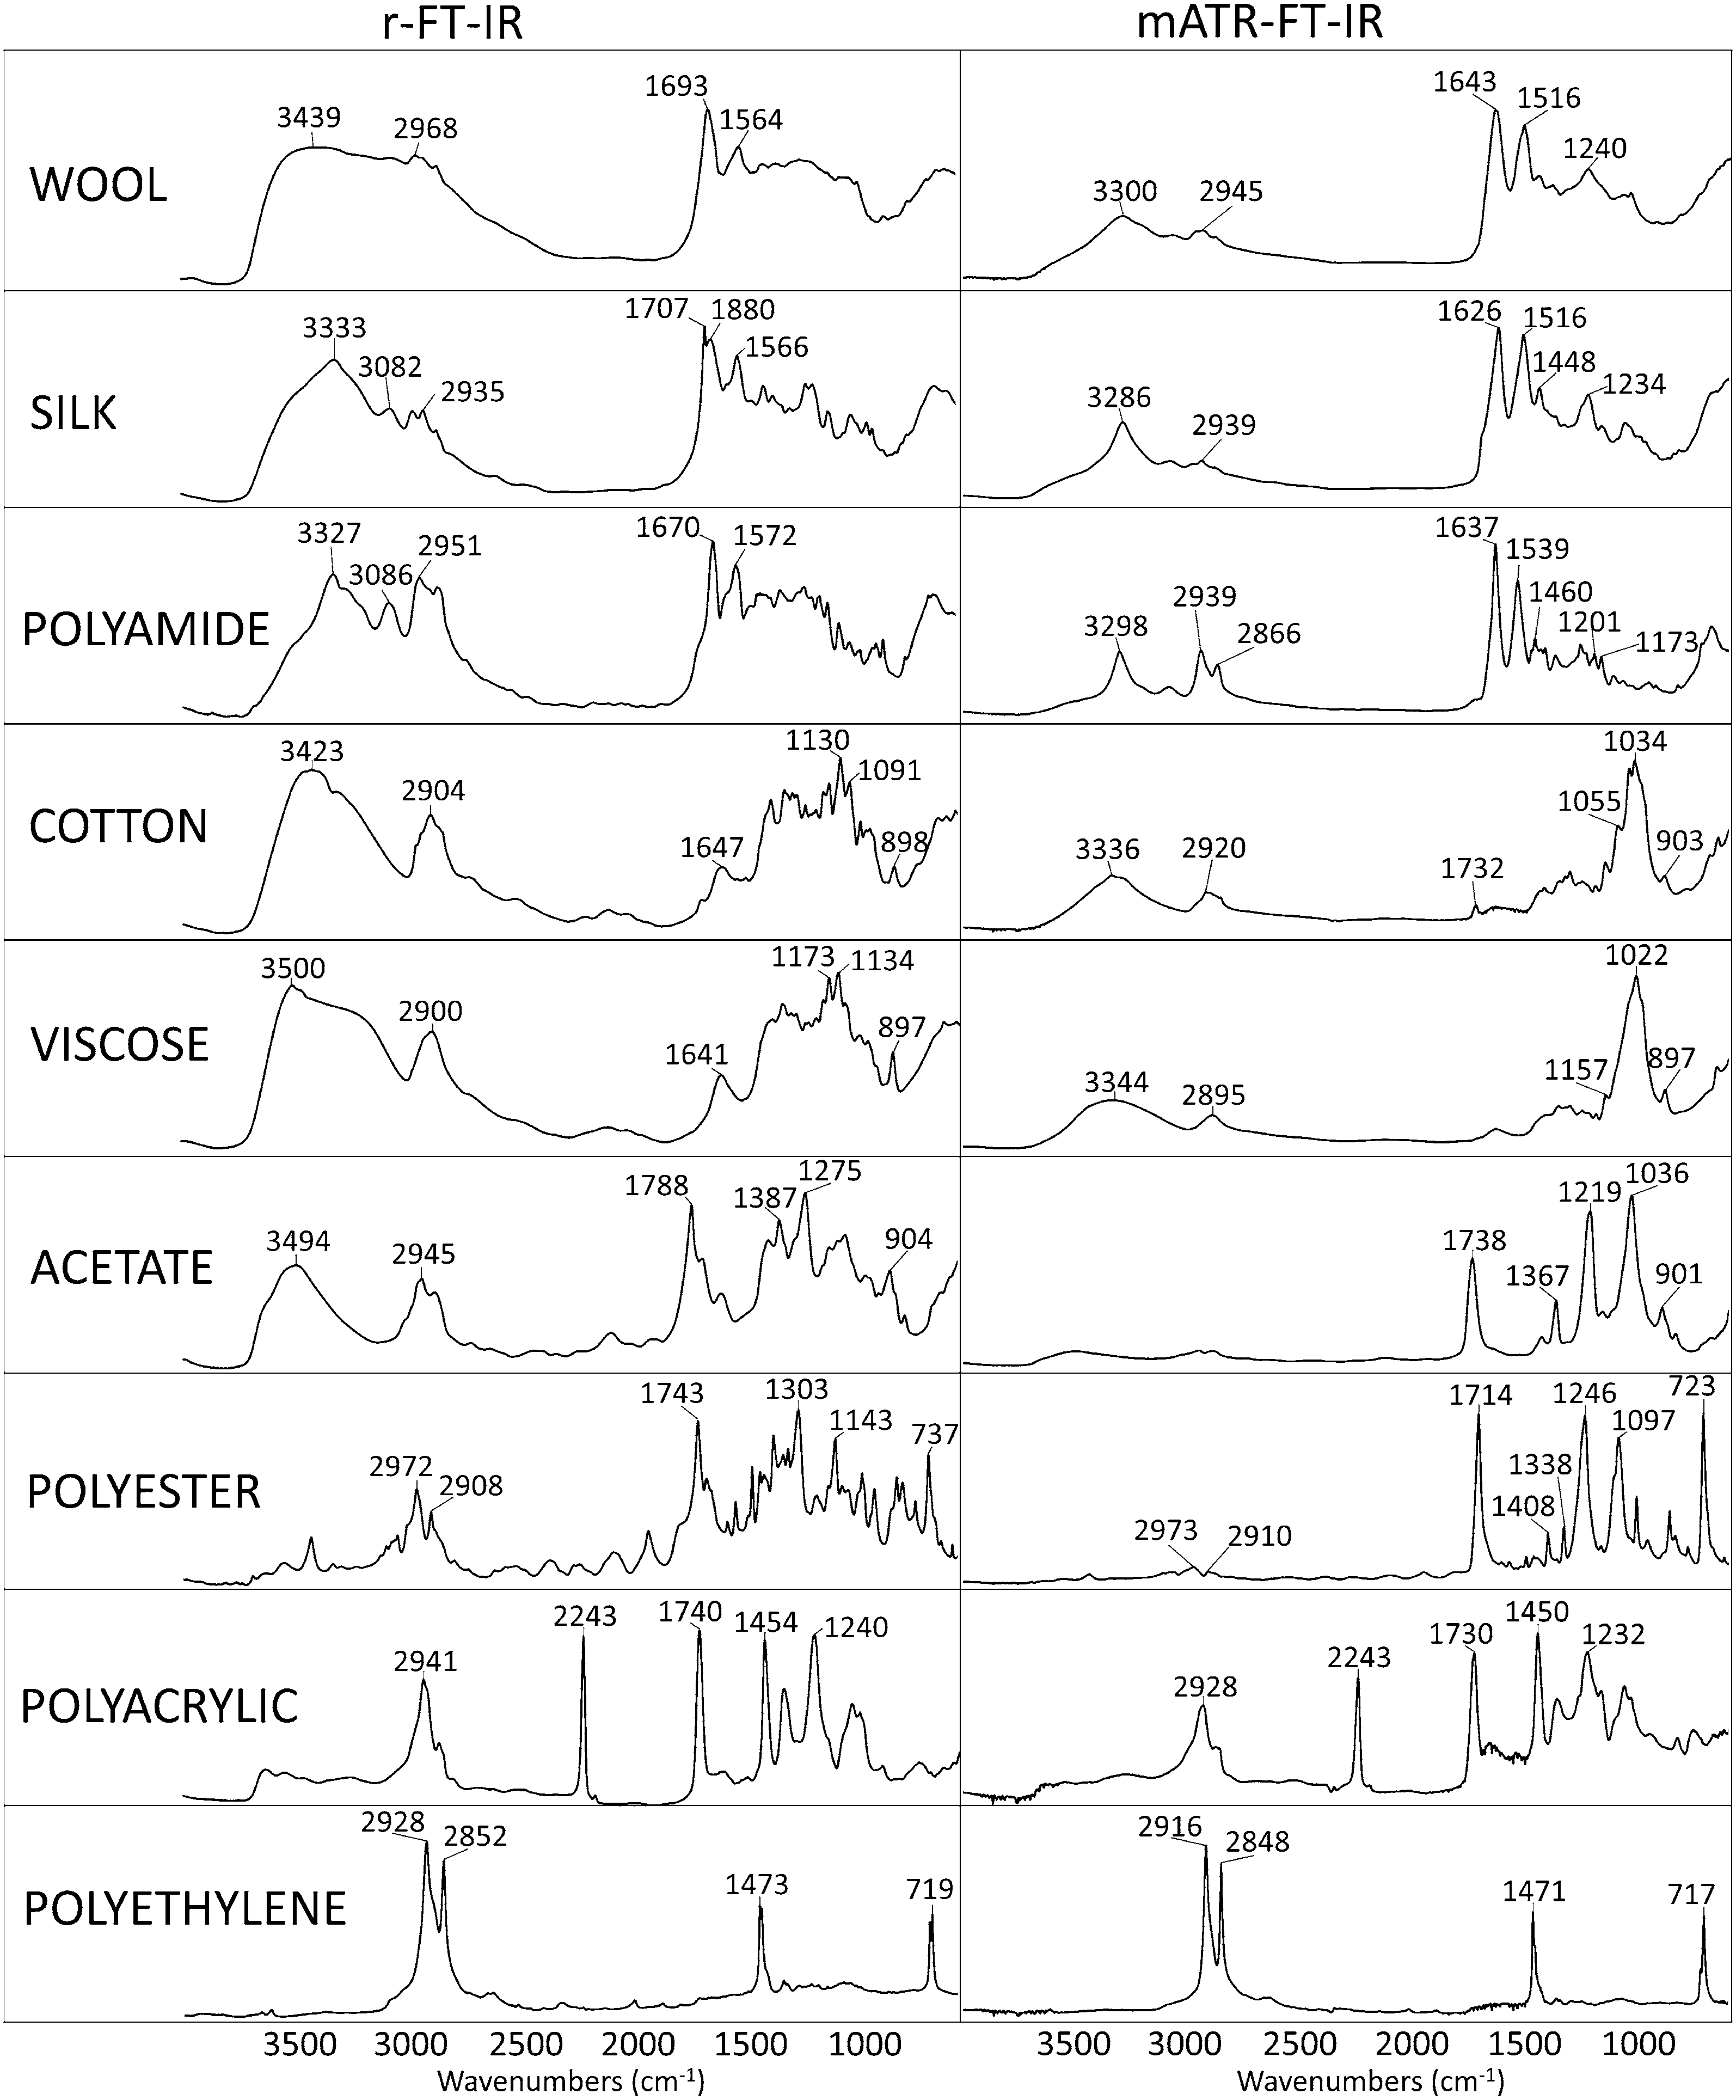
\includegraphics{images/1e7c6525-a9ac-4ff7-a4ff-b7128f317966-ufig1_comparison.png}}{}
\makeatother 
\caption{{r-FT-IR and mATR-FT-IR spectra of most common textile fibers. Spectra in figure represent normalized and averaged results of each. The vertical axis represents absorbance. \unskip~\protect\cite{693772:16533873}}}
\label{f-cbfac61d0782}
\end{figure*}
\egroup
Peets et al. report a table (Table~\ref{tw-524706f5cbef}), which compares the used FTIR spectroscopy characterization techniques for textile samples. The reflectance mode has the advantage of being non-invasive and non-destructive, especially in the case of valuable/fragile samples. However, r-FTIR does not work well with uneven surfaces, as less radiation is reflected into the detector. To compensate the drawbacks, the authors suggest using a higher number of scans, and a larger measurement area/aperture\unskip~\cite{693772:16533873}.


\begin{table*}[!htbp]
\caption{{Comparison of different FT-IR approaches for analyzing textile fibers \unskip~\protect\cite{693772:16533873}} }
\label{tw-524706f5cbef}
\def\arraystretch{1}
\ignorespaces 
\centering 
\begin{tabulary}{\linewidth}{LLL}
\tbltoprule Textile sample type/property & ATR-FT-IR spectrometer & r-FT-IR microspectrometer Non-contact\\
\tblmidrule 
Fragile sample &
  Applying pressure can damage the sample. High pressure should not be applied; spectrum quality might decrease. &
  Non-contact approach. \mbox{}\protect\newline Enables analyzing the sample with- out any alteration.\\
Thick sample &
  Penetration depth is few \ensuremath{\mu }m to few tens of \ensuremath{\mu }m. Fibers inside the fabric are not likely missed. &
  Spectrum is recorded only from the surface. Fibers in the inner part of the thread might be missed.\\
Uneven sample surface &
  Not a problem if enough pressure is applied, but high pressure may damage the sample. &
  More difficult to get high-quality spectrum. Scattering from the surface is extensive.\\
Extraneous material on sample fib- ers (additives or contaminants) &
  Penetration depth is few to few tens of \ensuremath{\mu }m. Surface contamination can have influence on the spectrum. &
  Spectrum is recorded only from the surface. Extraneous material on the surface \mbox{}\protect\newline can completely mask some fiber's bands and show additional bands.\\
Very small thread (less than 10 individual fibers) &
  Quality of the spectrum can be poor. &
  Spectrum may be distorted if the measured area (aperture) is larger than the sample thread itself.\\
\tblbottomrule 
\end{tabulary}\par 
\end{table*}
It can be concluded that r-FT-IR is a suitable technique for quick, easy, non-destructive and non-invasive analysis of different types of textile samples\unskip~\cite{693772:16533873}.

\clearpage 
    

\bibliographystyle{blank}

\bibliography{\jobname}

\section*{Author biography}

\bioItem[images/bf0f1284-fa36-4678-a9e7-05671376e50c-umeitesm]{Antonio Osamu Katagiri Tanaka}{ .

MNT16

A01212611}
\printBio 

\end{document}
